%\VignetteIndexEntry{An Introduction to the BPR method}
%\VignetteKeywords{BPR, methylation, gene expression}
%\VignettePackage{BPRMeth}
%\VignetteEngine{knitr::knitr}

\documentclass{article}\usepackage[]{graphicx}\usepackage[usenames,dvipsnames]{color}
%% maxwidth is the original width if it is less than linewidth
%% otherwise use linewidth (to make sure the graphics do not exceed the margin)
\makeatletter
\def\maxwidth{ %
  \ifdim\Gin@nat@width>\linewidth
    \linewidth
  \else
    \Gin@nat@width
  \fi
}
\makeatother

\definecolor{fgcolor}{rgb}{0.345, 0.345, 0.345}
\newcommand{\hlnum}[1]{\textcolor[rgb]{0.686,0.059,0.569}{#1}}%
\newcommand{\hlstr}[1]{\textcolor[rgb]{0.192,0.494,0.8}{#1}}%
\newcommand{\hlcom}[1]{\textcolor[rgb]{0.678,0.584,0.686}{\textit{#1}}}%
\newcommand{\hlopt}[1]{\textcolor[rgb]{0,0,0}{#1}}%
\newcommand{\hlstd}[1]{\textcolor[rgb]{0.345,0.345,0.345}{#1}}%
\newcommand{\hlkwa}[1]{\textcolor[rgb]{0.161,0.373,0.58}{\textbf{#1}}}%
\newcommand{\hlkwb}[1]{\textcolor[rgb]{0.69,0.353,0.396}{#1}}%
\newcommand{\hlkwc}[1]{\textcolor[rgb]{0.333,0.667,0.333}{#1}}%
\newcommand{\hlkwd}[1]{\textcolor[rgb]{0.737,0.353,0.396}{\textbf{#1}}}%

\usepackage{framed}
\makeatletter
\newenvironment{kframe}{%
 \def\at@end@of@kframe{}%
 \ifinner\ifhmode%
  \def\at@end@of@kframe{\end{minipage}}%
  \begin{minipage}{\columnwidth}%
 \fi\fi%
 \def\FrameCommand##1{\hskip\@totalleftmargin \hskip-\fboxsep
 \colorbox{shadecolor}{##1}\hskip-\fboxsep
     % There is no \\@totalrightmargin, so:
     \hskip-\linewidth \hskip-\@totalleftmargin \hskip\columnwidth}%
 \MakeFramed {\advance\hsize-\width
   \@totalleftmargin\z@ \linewidth\hsize
   \@setminipage}}%
 {\par\unskip\endMakeFramed%
 \at@end@of@kframe}
\makeatother

\definecolor{shadecolor}{rgb}{.97, .97, .97}
\definecolor{messagecolor}{rgb}{0, 0, 0}
\definecolor{warningcolor}{rgb}{1, 0, 1}
\definecolor{errorcolor}{rgb}{1, 0, 0}
\newenvironment{knitrout}{}{} % an empty environment to be redefined in TeX

\usepackage{alltt}

\RequirePackage{/usr/local/lib/R/site-library/BiocStyle/resources/tex/Bioconductor}

\AtBeginDocument{\bibliographystyle{/usr/local/lib/R/site-library/BiocStyle/resources/tex/unsrturl}}


\bioctitle[BPRMeth: Methylation features for clustering and prediction]{BPRMeth: Higher order methylation features for clustering and prediction in epigenomic studies}
\author{Chantriolnt-Andreas Kapourani\footnote{C.A.Kapourani@ed.ac.uk or kapouranis.andreas@gmail.com}}
\date{Modified: 1 August, 2016. Compiled: \today}
\IfFileExists{upquote.sty}{\usepackage{upquote}}{}
\begin{document}

\maketitle

\tableofcontents


%%
% Introduction section
%%
\section{Introduction}
DNA methylation is an intensely studied epigenetic mark, yet its functional role is incompletely understood. Attempts to quantitatively associate average DNA methylation to gene expression yield poor correlations outside of the well-understood methylation-switch at CpG islands.

Here we use probabilistic machine learning to extract higher order features associated with the methylation profile across a defined region. These features quantitate precisely notions of shape of a methylation profile, capturing spatial correlations in DNA methylation across genomic regions.  Using these higher order features across promoter-proximal regions, we are able to construct a powerful machine learning predictor of gene expression.


%%
% Background section
%%
\section{Background}
DNA methylation data produced by High-Throughput Sequencing (HTS) technology can be modelled with a Binomial distribution:
\begin{equation}
  m \sim \mathcal{B}inom(t, p)
\end{equation}

In practical studies we are interested in learning the methylation patterns of genomic regions which can be represented by an observation vector $\mathbf{y}$. Let $f(x) = \Phi \big(g(x)\big)$ be a latent function representing the methylation profiles and $g(x)$ be of the form:
\begin{equation}\label{eq-basis}
	 g(x) = \sum\limits_{j=0}^{M-1} w_{j} h_{j}(x)
\end{equation}
where $h_{j}(\cdot)$ can be any basis function, e.g. Radial Basis Function (RBF), and $w_{j}$ are the coefficients for each basis.

Given $f(x)$ the observations $y_{l}$ for each CpG site are i.i.d. Binomial variables, so we can define the joint log-likelihood in factorised form:
\begin{equation} \label{eq:bpr-likelihood}
 \log p(\mathbf{y} | f) = \sum\limits_{l = 1}^{L} \log \bigg( \mathcal{B}inom\big(m_{l} | t_{l}, \Phi(g(x_{l}))\big) \bigg)
\end{equation}
We refer to this observation model as the Binomial Probit Regression (BPR) likelihood function. \emph{Figure \ref{fig:model-performance}} shows the process of learning the methylation profile for a specific promoter region using the BPR model. For a more detailed explanation of the statistical method, see \cite{Kapourani2016}.

\begin{figure}[!ht]
\centerline{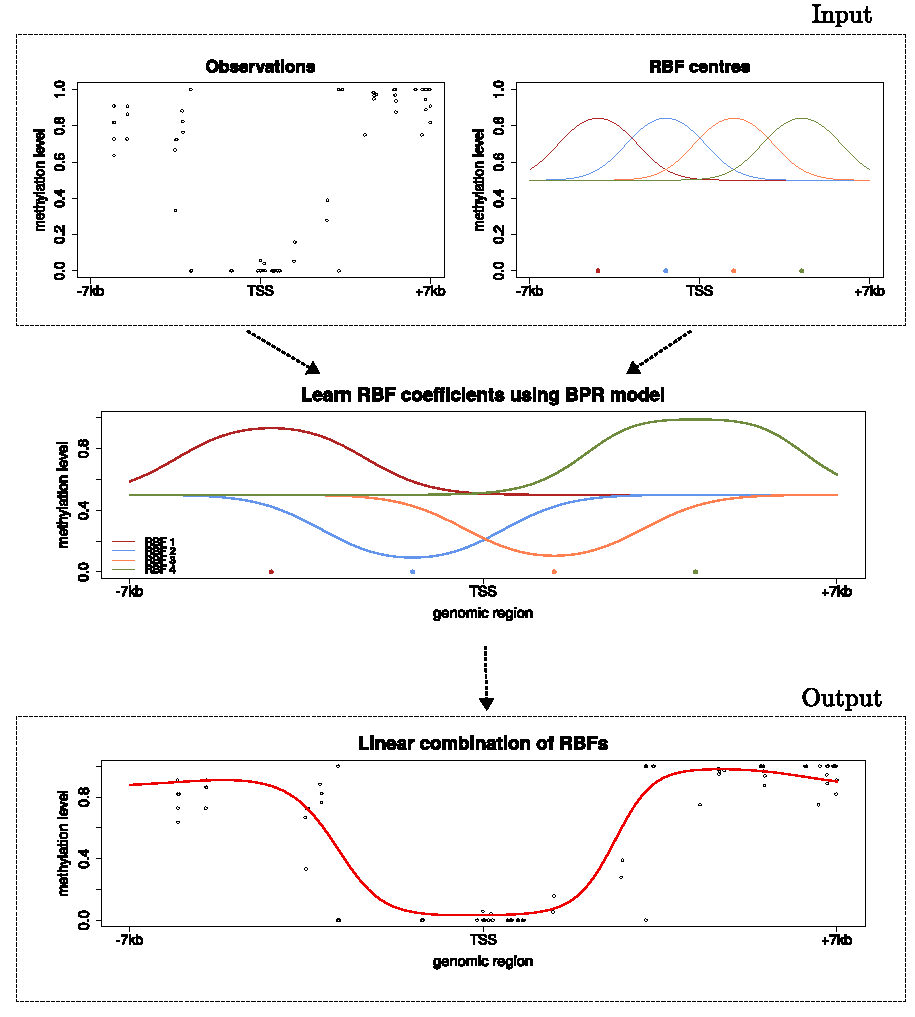
\includegraphics[width=0.66\textwidth]{model-bpr}}
\caption{\small{Illustration of the process for learning methylation profiles using the BPR model. The inputs to the model are the observed methylation levels of the CpGs across the promoter region, plus the number, with their corresponding centres, of the Radial Basis Functions (RBFs), which in this example are chosen to be four. Using this information the BPR model will learn the optimal coefficients for each RBF using maximum likelihood. Finally, we obtain the underlying methylation profile by a linear combination of the fitted RBFs. One should note that the higher the number of RBFs the better the resolution for the methylation profile.}}
\label{fig:model-performance}
\end{figure}


%%
% Analysis Pipeline section
%%
\section{Analysis Pipeline}

%%
% Sample data section
%%
\subsection{Sample data}
To illustrate the functions of the \verb|BPRMeth| package we will use real datasets that are publicly available from the ENCODE project consortium \cite{Dunham2012}. More specifically we will focus on the K562 immortalized cell line, with GEO: GSE27584 for the RRBS data and GEO: GSE33480 for the RNA-Seq data. We will use directly the preprocessed files, however, we should note that we have converted the RNA-Seq data from \verb|.gtf| to \verb|.bed| format using the \verb|bedops| tool (\href{http://bedops.readthedocs.io} {http://bedops.readthedocs.io}). We have kept only the protein coding genes, and for the purpose of this vignette we focus only on \verb|chr12| and \verb|chr13|. Full details of where to download the data and how to preprocess them are included in the Supplementary Material of \cite{Kapourani2016}.


%%
% Read HTS data section
%%
\subsection{Import and read HTS files}
Due to its general approach, the BPR method can be applied both in RRBS and WGBS methylation datasets, provided that we have information about the methylated and unmethylated reads in each CpG location.

The \verb|BPRMeth| package provides methods for reading files generated from HTS experiments with specific formats. For the formats provided by the ENCODE datasets described above; we have implemented \Rfunction{process\_haib\_caltech\_wrap}, which is a wrapper function for performing the preprocessing and obtaining the final objects for downstream analysis. The user can implement his own methods for reading files with different formats, provided that he can create an object similar to what is described below. First, we load and attach the package and then we obtain the paths for the sample RRBS and RNA-Seq files with the following commands:
\begin{kframe}
\begin{alltt}
\hlkwd{library}\hlstd{(BPRMeth)}
\hlstd{rrbs_file} \hlkwb{<-} \hlkwd{system.file}\hlstd{(}\hlstr{"extdata"}\hlstd{,} \hlstr{"rrbs.bed"}\hlstd{,} \hlkwc{package} \hlstd{=} \hlstr{"BPRMeth"}\hlstd{)}
\hlstd{rnaseq_file} \hlkwb{<-} \hlkwd{system.file}\hlstd{(}\hlstr{"extdata"}\hlstd{,} \hlstr{"rnaseq.bed"}\hlstd{,} \hlkwc{package} \hlstd{=} \hlstr{"BPRMeth"}\hlstd{)}
\end{alltt}
\end{kframe}

Then, we process both files to obtain a \verb|processHTS| object which will be used for downstream analysis:
\begin{kframe}
\begin{alltt}
\hlcom{# Preprocess both RRBS and RNA-Seq files}
\hlstd{HTS_data} \hlkwb{<-} \hlkwd{process_haib_caltech_wrap}\hlstd{(rrbs_file, rnaseq_file)}
\end{alltt}
\end{kframe}

Among other information, the \verb|processHTS| object contains the following important slots:
\begin{enumerate}
\item{A \Rfunction{list} where each entry corresponds to a different promoter methylation region, accessible with \textbf{methyl\_region}. \\ More specifically, each methylation promoter region is an $L_{i} \times 3$ dimensional matrix, where $L_{i}$ denotes the number of CpGs found in region $i$. The columns contain the following information:
\begin{itemize}
\item{ 1st column: Contains the locations of CpGs relative to TSS. Note that the actual locations are scaled to the (-1, 1) region. }
\item{ 2nd column: Contains the total reads of each CpG in the corresponding location.}
\item{ 3rd column: Contains the methylated reads each CpG in the corresponding location.}
\end{itemize} }
\item{A \Rfunction{vector} with the corresponding log2 transformed gene expression levels for each promoter region, accessible with \textbf{gex}.}
\item{A \Biocpkg{GRanges} object storing the RNA-Seq data together with annotation information for each promoter region, accessible with \textbf{rna\_data}.}
\end{enumerate}

Now, we give examples on how to access these information on the sample data described in the previous section. Initially, we can access the $16th$ promoter methylation region as follows:
\begin{knitrout}
\definecolor{shadecolor}{rgb}{0.969, 0.969, 0.969}\color{fgcolor}\begin{kframe}
\begin{alltt}
\hlstd{HTS_data}\hlopt{$}\hlstd{methyl_region[[}\hlnum{16}\hlstd{]]}
\end{alltt}
\begin{verbatim}
##              [,1] [,2] [,3]
##  [1,] -0.65185714    4    2
##  [2,]  0.02985714    4    0
##  [3,]  0.03128571    4    0
##  [4,]  0.03157143    4    0
##  [5,]  0.03285714    4    4
##  [6,]  0.03714286   38    0
##  [7,]  0.03942857   38    1
##  [8,]  0.03985714   38    0
##  [9,]  0.04014286   38    2
## [10,]  0.04128571   38    0
## [11,]  0.04185714   38    4
## [12,]  0.76028571    4    1
## [13,]  0.95685714   85   52
## [14,]  0.96028571   85   21
\end{verbatim}
\end{kframe}
\end{knitrout}

Below we show the log2 transformed gene expression levels for the first 10 promoter regions:
\begin{knitrout}
\definecolor{shadecolor}{rgb}{0.969, 0.969, 0.969}\color{fgcolor}\begin{kframe}
\begin{alltt}
\hlkwd{head}\hlstd{(HTS_data}\hlopt{$}\hlstd{gex,} \hlnum{10}\hlstd{)}
\end{alltt}
\begin{verbatim}
##  [1] -3.321928  1.587480  1.792014  2.695450 -2.708765  6.715633  2.109909  1.618953
##  [9] -3.321928 -3.321928
\end{verbatim}
\end{kframe}
\end{knitrout}

Finally, the RNA-Seq data which are stored in a \Biocpkg{GRanges} object, can be accessed as follows:
\begin{knitrout}
\definecolor{shadecolor}{rgb}{0.969, 0.969, 0.969}\color{fgcolor}\begin{kframe}
\begin{alltt}
\hlstd{HTS_data}\hlopt{$}\hlstd{rna_data}
\end{alltt}
\begin{verbatim}
## GRanges object with 334 ranges and 3 metadata columns:
##         seqnames                 ranges strand |      ensembl_id   gene_name gene_fpkm
##            <Rle>              <IRanges>  <Rle> |     <character> <character> <numeric>
##     [1]    chr12     [ 569529,  672675]      + | ENSG00000139044    B4GALNT3 0.0000000
##     [2]    chr12     [ 752147,  755044]      + | ENSG00000177406  AC021054.1 2.9052400
##     [3]    chr12     [1021242, 1058888]      - | ENSG00000002016       RAD52 3.3629800
##     [4]    chr12     [1675158, 1703331]      - | ENSG00000171823      FBXL14 6.3775600
##     [5]    chr12     [1901122, 2027870]      - | ENSG00000151062    CACNA2D4 0.0529609
##     ...      ...                    ...    ... .             ...         ...       ...
##   [330]    chr13 [114303172, 114312501]      - | ENSG00000186009       ATP4B   0.00000
##   [331]    chr13 [114321469, 114438724]      + | ENSG00000185974        GRK1   0.00000
##   [332]    chr13 [114462215, 114514926]      + | ENSG00000184497      FAM70B   0.00000
##   [333]    chr13 [114523523, 114567046]      - | ENSG00000183087        GAS6   8.55437
##   [334]    chr13 [114747193, 114898095]      - | ENSG00000185989       RASA3  15.20510
##   -------
##   seqinfo: 2 sequences from an unspecified genome; no seqlengths
\end{verbatim}
\end{kframe}
\end{knitrout}

The package provides implementation for specific parts of the preprocessing steps described above which can be seen by typing \Rfunction{process\_haib\_caltech\_wrap} on the R console. If the user has files with different formats, he can implement his own functions for reading the data and then combine them with the simple functions present in the BPRMeth package, in order to obtain an object similar to \verb|processHTS|, which should have the slots described above.


%%
% Predict expression section
%%
\subsection{Predict gene expression}
After preprocessing the HTS data, we have the following number of unique protein-coding genes belonging in chr12 and chr13:
\begin{knitrout}
\definecolor{shadecolor}{rgb}{0.969, 0.969, 0.969}\color{fgcolor}\begin{kframe}
\begin{alltt}
\hlcom{# Obtain the number of gene promoters}
\hlkwd{length}\hlstd{(HTS_data}\hlopt{$}\hlstd{gex)}
\end{alltt}
\begin{verbatim}
## [1] 334
\end{verbatim}
\end{kframe}
\end{knitrout}

Learning the methylation profiles is equivalent to optimizing the model parameters $\mathbf{w}$ described in Eq. \ref{eq-basis}. These parameters can be considered as the extracted features which quantitate precisely notions of shape of a methylation profile.

\subsubsection{Create basis objects}
For each promoter region, we will learn its methylation profile using the BPR model with a specified number of Radial Basis Functions (RBFs) $M$. For a single input variable $x$, the RBF takes the form $h_{j}(x) = exp(-\gamma || x - \mu_{j} ||^2)$, where $\mu_{j}$ denotes the location of the $j^{th}$ basis function in the input space and $\gamma$ controls the spatial scale. The case when $M = 0$ is equivalent to learning the average methylation level for the given region (i.e. learn a constant function).

For our running example, we will create two RBF objects, one with 9 basis functions and the other with 0 basis functions denoting the mean methylation level approach:
\begin{knitrout}
\definecolor{shadecolor}{rgb}{0.969, 0.969, 0.969}\color{fgcolor}\begin{kframe}
\begin{alltt}
\hlcom{# Create basis object with 9 RBFs}
\hlstd{basis_profile} \hlkwb{<-} \hlkwd{create_rbf_object}\hlstd{(}\hlkwc{M} \hlstd{=} \hlnum{9}\hlstd{)}

\hlcom{# Create basis object with 0 RBFs, i.e. constant function}
\hlstd{basis_mean} \hlkwb{<-} \hlkwd{create_rbf_object}\hlstd{(}\hlkwc{M} \hlstd{=} \hlnum{0}\hlstd{)}
\end{alltt}
\end{kframe}
\end{knitrout}

The \Rfunction{rbf} object contains information such as the centre locations $\mu_{j}$ and the value of the spatial scale parameter $\gamma$:
\begin{knitrout}
\definecolor{shadecolor}{rgb}{0.969, 0.969, 0.969}\color{fgcolor}\begin{kframe}
\begin{alltt}
\hlcom{# Show the slots of the 'rbf' object}
\hlstd{basis_profile}
\end{alltt}
\begin{verbatim}
## $M
## [1] 9
## 
## $mus
## [1] -0.8 -0.6 -0.4 -0.2  0.0  0.2  0.4  0.6  0.8
## 
## $gamma
## [1] 20.25
## 
## $eq_spaced_mus
## [1] TRUE
## 
## $whole_region
## [1] TRUE
## 
## attr(,"class")
## [1] "rbf"
\end{verbatim}
\end{kframe}
\end{knitrout}
The $\gamma$ is computed by the number of basis M, however the user can tune it according to his liking. Except from RBF basis, the \verb|BPRMeth| pacakge provides polynomial basis which can be created with the \Rfunction{create\_polynomial\_object} function.

\subsubsection{Learn methylation profiles and make predictions}
We can now optimize the BPR likelihood function and extract the features $\mathbf{w}_{i}$ for each promoter region. To quantitatively predict expression at each region, we construct a regression model by taking as input the higher-order methylation features learned from the BPR model. In addition to these features, we consider two supplementary sources of information: (1) the goodness of fit in RMSE and (2) the CpG density. For our analysis an SVM regression model is considered. We will use $70\%$ of the data for training, and we will test the model's performance on the remaining $30\%$.

All the aforementioned steps are assembled in the \Rfunction{bpr\_predict\_wrap} wrapper function, which returns a \verb|bpr_predict| object.
\begin{knitrout}
\definecolor{shadecolor}{rgb}{0.969, 0.969, 0.969}\color{fgcolor}\begin{kframe}
\begin{alltt}
\hlcom{# Set seed for reproducible results}
\hlkwd{set.seed}\hlstd{(}\hlnum{1234}\hlstd{)}


\hlcom{# Perform predictions using methylation profiles}
\hlstd{res_profile} \hlkwb{<-} \hlkwd{bpr_predict_wrap}\hlstd{(}\hlkwc{x} \hlstd{= HTS_data}\hlopt{$}\hlstd{methyl_region,} \hlkwc{y} \hlstd{= HTS_data}\hlopt{$}\hlstd{gex,}
                                \hlkwc{basis} \hlstd{= basis_profile,} \hlkwc{fit_feature} \hlstd{=} \hlstr{"RMSE"}\hlstd{,}
                                \hlkwc{cpg_dens_feat} \hlstd{=} \hlnum{TRUE}\hlstd{,} \hlkwc{is_parallel} \hlstd{=} \hlnum{FALSE}\hlstd{,}
                                \hlkwc{is_summary} \hlstd{=} \hlnum{FALSE}\hlstd{)}

\hlcom{# Perform predictions using mean methylation level}
\hlstd{res_mean} \hlkwb{<-} \hlkwd{bpr_predict_wrap}\hlstd{(}\hlkwc{x} \hlstd{= HTS_data}\hlopt{$}\hlstd{methyl_region,} \hlkwc{y} \hlstd{= HTS_data}\hlopt{$}\hlstd{gex,}
                             \hlkwc{basis} \hlstd{= basis_mean,} \hlkwc{is_parallel} \hlstd{=} \hlnum{FALSE}\hlstd{,}
                             \hlkwc{is_summary} \hlstd{=} \hlnum{FALSE}\hlstd{)}
\end{alltt}
\end{kframe}
\end{knitrout}

We can now compare the Pearson's correlation coefficient $r$ for both models and observe that the higher-order methylation features achieve test correlations twice as large as previously reported when using average methylation levels.
\begin{knitrout}
\definecolor{shadecolor}{rgb}{0.969, 0.969, 0.969}\color{fgcolor}\begin{kframe}
\begin{alltt}
\hlcom{# Test errors for methylation profiles, PCC = Pearson's r}
\hlstd{res_profile}\hlopt{$}\hlstd{test_errors}\hlopt{$}\hlstd{pcc}
\end{alltt}
\begin{verbatim}
## [1] 0.7160231
\end{verbatim}
\begin{alltt}
\hlcom{# Test errors for mean methylation levels}
\hlstd{res_mean}\hlopt{$}\hlstd{test_errors}\hlopt{$}\hlstd{pcc}
\end{alltt}
\begin{verbatim}
## [1] 0.2953251
\end{verbatim}
\end{kframe}
\end{knitrout}

Figure \ref{figure/figureexample-1} shows an example promoter region together with the fitted methylation profiles.
\begin{knitrout}
\definecolor{shadecolor}{rgb}{0.969, 0.969, 0.969}\color{fgcolor}\begin{kframe}
\begin{alltt}
\hlcom{# Choose promoter region 21 -> i.e. LEPREL2 gene}
\hlstd{gene_name} \hlkwb{<-} \hlstd{HTS_data}\hlopt{$}\hlstd{rna_data}\hlopt{$}\hlstd{gene_name[}\hlnum{21}\hlstd{]}
\hlkwd{plot_fitted_profiles}\hlstd{(}\hlkwc{region} \hlstd{=} \hlnum{21}\hlstd{,} \hlkwc{X} \hlstd{= HTS_data}\hlopt{$}\hlstd{methyl_region,} \hlkwc{fit_prof} \hlstd{= res_profile,}
                     \hlkwc{fit_mean} \hlstd{= res_mean,} \hlkwc{title} \hlstd{=} \hlkwd{paste0}\hlstd{(}\hlstr{"Gene "}\hlstd{, gene_name))}
\end{alltt}
\end{kframe}
\end{knitrout}
\incfig{figure/figureexample-1}{0.8\textwidth}{Methylation pattern for the LEPREL2 gene over $\pm7kb$ promoter region.}
{The points represent the DNA methylation level of each CpG site. The shape of the methylation profiles is captured by the red curve, whereas the orange dashed line denotes the mean methylation level.}

Figure \ref{figure/figureexample2-1} shows a scatter plot of the predicted and measured expression values for the \verb|chr12| and \verb|chr13| of the K562 cell line.
\begin{knitrout}
\definecolor{shadecolor}{rgb}{0.969, 0.969, 0.969}\color{fgcolor}\begin{kframe}
\begin{alltt}
\hlkwd{par}\hlstd{(}\hlkwc{mfrow}\hlstd{=}\hlkwd{c}\hlstd{(}\hlnum{1}\hlstd{,}\hlnum{2}\hlstd{))}
\hlkwd{plot_scatter_gex}\hlstd{(}\hlkwc{bpr_predict_obj} \hlstd{= res_profile)}
\hlkwd{plot_scatter_gex}\hlstd{(}\hlkwc{bpr_predict_obj} \hlstd{= res_mean,} \hlkwc{main_lab} \hlstd{=} \hlstr{"Mean Methylation"}\hlstd{)}
\end{alltt}
\end{kframe}
\end{knitrout}
\incfig{figure/figureexample2-1}{0.98\textwidth}{Quantitative relationship between DNA methylation patterns and gene expression.}{Scatter plots of predicted versus measured (log2-transformed) gene expression values: using the BPR model and extracting higher-order features \emph{(left)}, and using the average methylation level \emph{right} as input to the SVM regression model. Each shaded blue dot represents a different gene. The red dashed line indicates the linear fit between the predicted and measured expression values.}

%%
% Cluster profiles section
%%
\subsection{Cluster methylation profiles}
Another application of the BPR model is to use the higher-order methylation features to cluster DNA methylation patterns across promoter-proximal regions and examine whether distinct methylation profiles are associated to different gene expression levels. To cluster methylation profiles, we consider a mixture modelling approach and we apply the EM algorithm to estimate the model parameters.

The \verb|BPRMeth| package provides the \Rfunction{bpr\_cluster\_wrap} function for performing the clustering process, where the user needs to provide the number of clusters $K$, the methylation regions and a basis object. Since we are interested in capturing broader similarities between profiles rather than fine details, we will model the methylation profiles at a slightly lower resolution:
\begin{knitrout}
\definecolor{shadecolor}{rgb}{0.969, 0.969, 0.969}\color{fgcolor}\begin{kframe}
\begin{alltt}
\hlcom{# Set seed for reproducible results}
\hlkwd{set.seed}\hlstd{(}\hlnum{1234}\hlstd{)}
\hlcom{# Create basis object with 4 RBFs}
\hlstd{basis_obj} \hlkwb{<-} \hlkwd{create_rbf_object}\hlstd{(}\hlkwc{M} \hlstd{=} \hlnum{4}\hlstd{)}
\hlcom{# Set number of clusters K = 5}
\hlstd{K} \hlkwb{<-} \hlnum{5}
\hlcom{# Perform clustering}
\hlstd{res} \hlkwb{<-} \hlkwd{bpr_cluster_wrap}\hlstd{(}\hlkwc{x} \hlstd{= HTS_data}\hlopt{$}\hlstd{methyl_region,} \hlkwc{K} \hlstd{= K,} \hlkwc{basis} \hlstd{= basis_obj,}
                        \hlkwc{em_max_iter} \hlstd{=} \hlnum{15}\hlstd{,} \hlkwc{opt_itnmax} \hlstd{=} \hlnum{30}\hlstd{,} \hlkwc{is_parallel} \hlstd{=} \hlnum{FALSE}\hlstd{)}
\end{alltt}
\end{kframe}
\end{knitrout}

Figure \ref{figure/figureexample3-1} shows the fitted methylation profiles for each cluster.
\begin{knitrout}
\definecolor{shadecolor}{rgb}{0.969, 0.969, 0.969}\color{fgcolor}\begin{kframe}
\begin{alltt}
\hlkwd{par}\hlstd{(}\hlkwc{mfrow}\hlstd{=}\hlkwd{c}\hlstd{(}\hlnum{1}\hlstd{,}\hlnum{2}\hlstd{))}
\hlkwd{plot_cluster_prof}\hlstd{(}\hlkwc{bpr_cluster_obj} \hlstd{= res)}
\hlkwd{boxplot_cluster_gex}\hlstd{(}\hlkwc{bpr_cluster_obj} \hlstd{= res,} \hlkwc{gex} \hlstd{= HTS_data}\hlopt{$}\hlstd{gex)}
\end{alltt}
\end{kframe}
\end{knitrout}
\incfig{figure/figureexample3-1}{0.99\textwidth}{Clustering methylation profiles across promoter-proximal regions.}{\emph{(Left)} Five clustered methylation profiles over $\pm 7kb$ promoter region w.r.t. TSS in the direction of transcription. Each methylation profile is modelled using four RBFs. \emph{(Right)} Boxplots with the corresponding expression levels of the protein-coding genes assigned to each cluster. The colors match with the clustered methylation profiles shown on the left.}


%%
% SessionInfo section
%%
%\clearpage
\section{Session Info}
This vignette was compiled using:
\begin{knitrout}
\definecolor{shadecolor}{rgb}{0.969, 0.969, 0.969}\color{fgcolor}\begin{kframe}
\begin{alltt}
\hlkwd{sessionInfo}\hlstd{()}
\end{alltt}
\begin{verbatim}
## R version 3.3.1 (2016-06-21)
## Platform: x86_64-pc-linux-gnu (64-bit)
## Running under: Ubuntu 14.04.4 LTS
## 
## locale:
##  [1] LC_CTYPE=en_GB.UTF-8       LC_NUMERIC=C               LC_TIME=en_GB.UTF-8       
##  [4] LC_COLLATE=en_GB.UTF-8     LC_MONETARY=en_GB.UTF-8    LC_MESSAGES=en_GB.UTF-8   
##  [7] LC_PAPER=en_GB.UTF-8       LC_NAME=C                  LC_ADDRESS=C              
## [10] LC_TELEPHONE=C             LC_MEASUREMENT=en_GB.UTF-8 LC_IDENTIFICATION=C       
## 
## attached base packages:
## [1] stats4    parallel  stats     graphics  grDevices utils     datasets  methods  
## [9] base     
## 
## other attached packages:
## [1] BPRMeth_0.99.1       GenomicRanges_1.24.2 GenomeInfoDb_1.8.3   IRanges_2.6.1       
## [5] S4Vectors_0.10.2     BiocGenerics_0.18.0  knitr_1.13           colorout_1.1-2      
## 
## loaded via a namespace (and not attached):
##  [1] XVector_0.12.1      magrittr_1.5        zlibbioc_1.18.0     MASS_7.3-45        
##  [5] doParallel_1.0.10   plotmo_3.1.4        foreach_1.4.3       highr_0.6          
##  [9] stringr_1.0.0       tools_3.3.1         data.table_1.9.6    plotrix_3.6-3      
## [13] e1071_1.6-7         iterators_1.0.8     class_7.3-14        randomForest_4.6-12
## [17] assertthat_0.1      formatR_1.4         codetools_0.2-14    evaluate_0.9       
## [21] earth_4.4.4         stringi_1.1.1       compiler_3.3.1      TeachingDemos_2.10 
## [25] BiocStyle_2.0.2     chron_2.3-47
\end{verbatim}
\end{kframe}
\end{knitrout}

%%
% Acknowledgements section
%%
\section{Acknowledgements}
This package was developed at the University of Edinburgh in the School of Informatics, with support from Guido
Sanguinetti.

This study was supported in part by the EPSRC Centre for Doctoral Training in Data Science, funded by the UK Engineering and Physical Sciences Research Council (grant EP/L016427/1) and the University of Edinburgh, and by the European Research Council through grant MLCS306999.

\bibliography{BPRMeth_vignette}

\end{document}
